\chapter{绪论}

\section{模式(字符串)匹配}

模式匹配(Pattern Matching, 简称PM), 一直以来都是计算机科学的核心问题之
一。 这里的“模式”特指字符串。 对于很多应用, 例如模式识
别 \cite{Yan2016}, \cite{Xiao2016}, 本体匹配 \cite{Xue2015}
\cite{Xue2016}, 文本分类 \cite{Tang2015} \cite{Zhang2016}, 系统安
全 \cite{Dien2014,Malhotra2016,Fan2016},入侵检测系
统 \cite{Kim2015,Arney2016,Sadotra2016,Lee2017} 等等, 模式匹配算法都是
最为基本而重要的操作。根据待匹配模式的数量,模式匹配技术可以分为两类:
单模式匹配(SPM)和多模式匹配(MPM)。

\begin{figure}[!h]
  \centering
  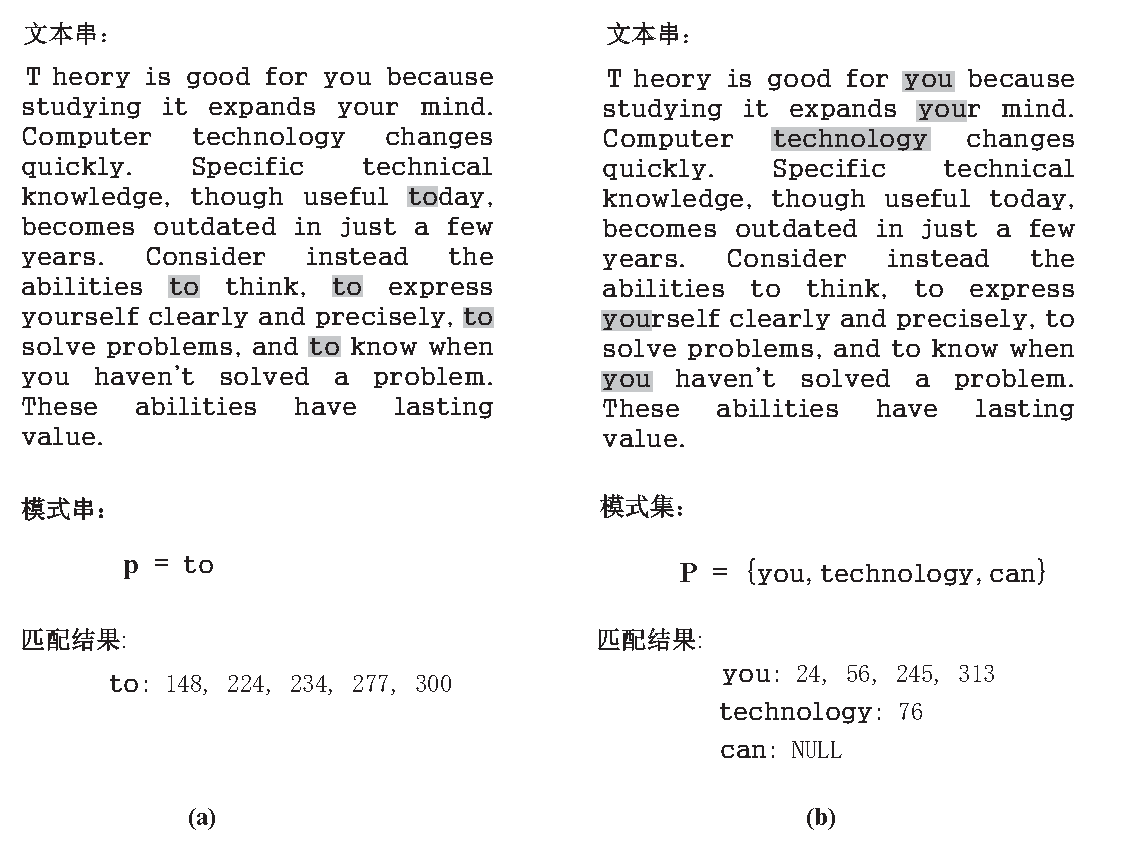
\includegraphics[height=8cm ,width=12cm]{figures/1_Introduction/SPM_MPM.eps}
  \caption{(A) 单模式匹配示例。(B) 多模式匹配示例。}
  \label{fig:SPM_MPM}
\end{figure}


\subsection{单模式匹配}

单模式匹配算法要求在文本串中寻找给定模式串的所有出现位置。如
图 \ref{fig:SPM_MPM } (A) 所示, 给定文本串与模式$to$, 经过匹配发现,模
式串$to$ 出现于文本串中的位置为: 148, 224, 234, 277, 300。

最简单的单模式匹配算法,需要对文本串中的每一个位置与模式串进行逐字符的
比较,一旦出现字符失配,将直接移动到文本串的下一个位置进行匹配。很明显,
当文本串的长度为$n$且模式串的长度为$m$时,这种简单的模式匹配算法的时间
复杂度为$O(m \cdot
n)$。当文本串形如$aaa \dots
a$及模式串为$aaab$时,将出现最坏情况。为此,有更加高效的单模式匹配算法
被提出,最著名的包括KMP \cite{Knuth1977}算法 和 BM \cite{Boyer1977} 算
法。下面将简单介绍这两种算法的主要思想。

1. \textbf{KMP(Knuth-Morris-Pratt)算法}

KMP算法的核心思想在于,一旦匹配失败,可以充分利用已经匹成功的子串信息,
让模式串向右移动尽可能多的位置。右移的距离是这样计算的:在已经匹配的模
式串子串中,找出最长的相同的前缀和后缀,然后向右移动使它们重叠。如
图\ref{fig:KMP}(A)所示,在当前匹配中,文本串中的位置10($i=10$)和模式串
中的位置8($j=8$)出现失配,根据已经匹配成功的子串即$abcdaabc$的信息:该
子串相等的最长前缀与最长后缀是$abc$, 将模式串向右移动使得这两部分相重合,
如图 \ref{fig:KMP} (B)
所示。此时,文本串中当前待匹配位置$i$不变,而模式串中当前待匹配位
置$j$变为3,分别从位置$i$和$j$开始对文本串和模式串进行逐字符比较。KMP算
法在匹配过程中,文本串中的当前匹配位置$i$永不减小,只是当匹配失败时,根
据模式串中的失配位置,来调整模式串中的下一次与文本串位置$i$相比较的位置。
因此,需要知道在失配时,下一次应当用模式串的哪个位置与文本串进行比较。
为此对模式串进行预处理,为其建立失配数组$Next$(如图 \ref{fig:KMP} (C)所
示),
如果当前在模式串的位置$j$失配时,下一次将用模式串的位置$Next[j]$来与文
本串进行比较,预处理过程的时间复杂度为$O(m)$($m$为模式串长度)。 由于匹
配过程中, 文本串中的位置$i$永不回溯,所以KMP算法的时间复杂度为$O(m+n)$
($n$为文本串长度)。

\begin{figure}[!h]
  \centering
  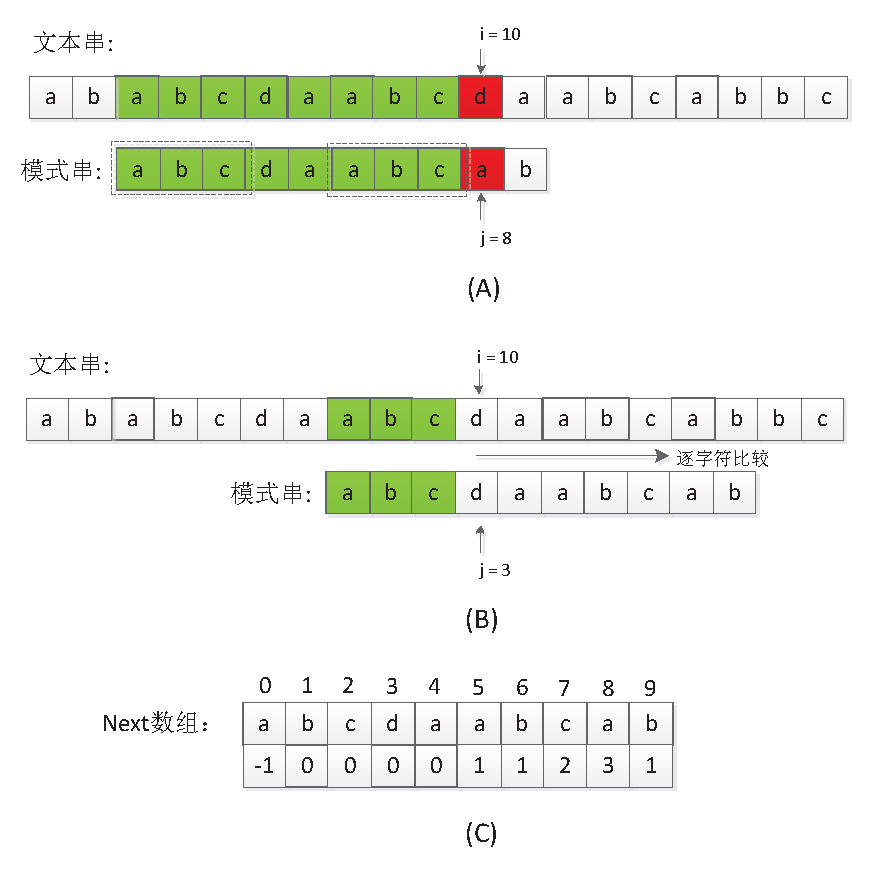
\includegraphics[height=10cm ,width=12cm]{figures/1_Introduction/KMP.eps}
  \caption{KMP算法示例。(A) 第一轮匹配。(B) 第二轮匹配。(C) 模式串
    的Next数组。}
  \label{fig:KMP}
\end{figure}


2. \textbf{BM(Boyer-Moore)算法}

尽管KMP算法具有线性的时间复杂度,可其实际的速度却并不快。在实际应用当中
(比如各类字处理软件中的字符串查找功能),最常用的单模式匹配算法是BM算
法 \cite{Boyer1977}, 及其诸多变体。BM算法最高效之处在于通过使用“坏字
符”规则,其可以快速跳过文本串中大量的不可能出现匹配的位置。如
图 \ref{fig:BM} (A) 所示,BM算法采用从右到左的方向对模式串与文本串进行
比较,由于第一次比较即失配且文本串中相应的字符$s$没有出现在模式串中,因
此可以将模式串整体向右移动到$s$的下一个字符处,然后再别从位
置13($i=13$)和位置6($j=6$),从右向左地对文本串和模式串进行比较,如
图 \ref{fig:BM} (B)
所示。由于再次失配,且文本串中的字符$p$出现于模式串中,因此将模式串向右
移动2个位置,使两个串中的$p$字符对齐,如图\ref{fig:BM}(C)所示。由于BM算
法在每次匹配失败时,都将根据文本串中的失配字符来移动模式串,因此需要对
整个字符集进行预处理构建坏字符表(表长为$|\Sigma|$,即字符集大小),当
匹配失败时用文本串中的失配字符作为索引来查找坏字符表,来决定需要将模式
串向后移动多少位。BM算法最坏情况的时间复杂度为$O(n \cdot m)$,但是在实
际中很少出现这样的情况。

\begin{figure}[!h]
  \centering
  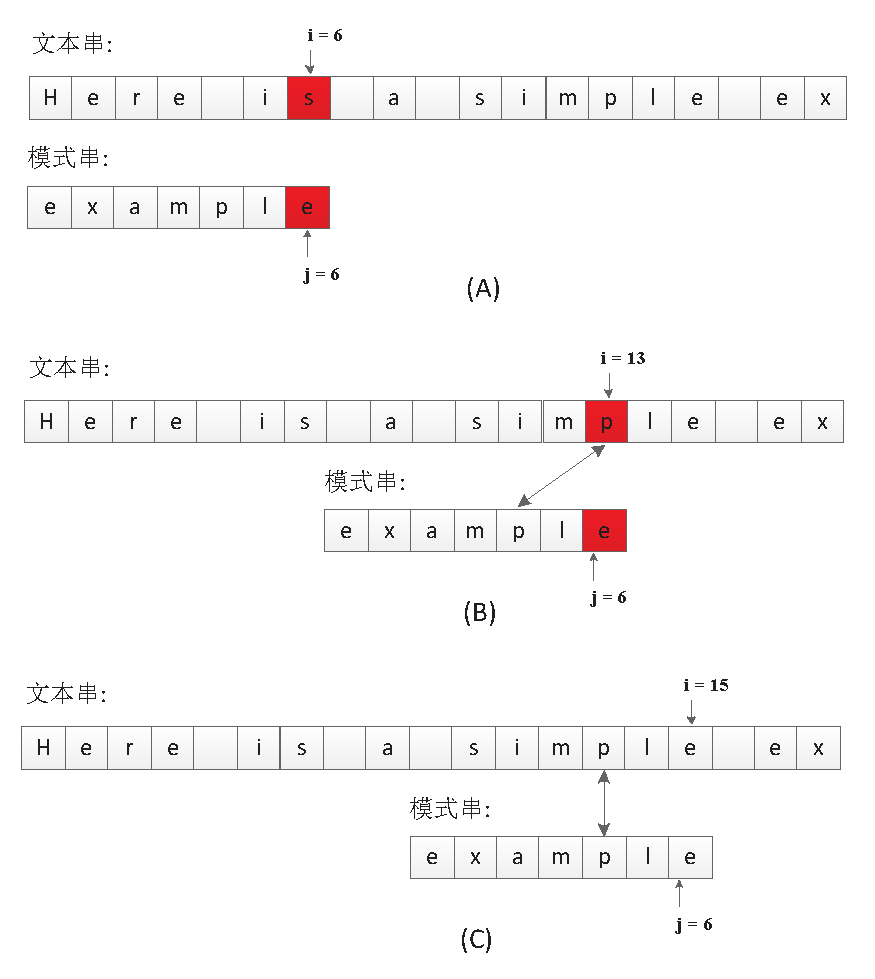
\includegraphics[height=10cm ,width=12cm]{figures/1_Introduction/BM.eps}
  \caption{BM算法示例。(A) 第一轮匹配。(B) 第二轮匹配。(C) 第三轮匹配。}
  \label{fig:KMP}
\end{figure}

\subsection{多模式匹配}

多模式匹配要求找出给定模式集中每一个模式串在文本串中的所有出现位置。如
图 \ref{fig:SPM_MPM} (B)
所示,给定模式集$P=\{can, you, technology\}$及文本串,通过多模式匹配发
现, 模式串$you$出现了4次, 模式串$technology$出现了1次, 模式串$can$在
文本串中没有出现。

目前,多模式匹配算法的主要流程是先对模式集进行预处理,构建合适的数据结
构来存储和组织模式集中的模式串,然后用构建好的数据结构和文本进行比较,
一次性找出所有模式集的出现位置。 比较著名的多模式匹配算法包括 AC
\cite{Aho1975} 和 WM \cite{Wu1994} 算法。

1. \textbf{AC(Aho-Corasick)算法}

AC算法是经典的多模式匹配算法,它是KMP算法在多模式环境下的推广,具有线性
时间复杂度。目前,各种AC算法的变体在实际当中被广泛应用。AC算法通过为模
式集构造一个有限状态自动机(DFA),然后将文本串中的每一个字符输入到自动机
中进行状态转移,来实现多模式匹配。图 \ref{fig:AC} 所示的是为模式
集$P=\{he, his, she, hers\}$ 所构造的AC自动机,图中实线箭头及对应字符表
示,在当前状态遇到该字符时应该跳转到的状态,虚线表示在当前状态无匹配字
符时,应该跳转到的状态,图中绿色的状态,表示匹配成功状态。 匹配时,AC算
法将从状态0开始,连续不断地读入文本串中的字符,并根据所读入的字符进行状
态跳转,一旦到达匹配成功状态,将输出匹配到的模式串。 举例说明,假设文本
串为$hers$, 初始状态为0, 第一个文本串字符为$h$, 则自动机将跳转到状态1;
下一个输入字符为$e$,
将跳转到状态2,同时成功匹配模式串$he$并将其输出;下一个字符为$r$,将跳
转到状态8;最后一个字符为$s$,跳转到状态9,并输入匹配成功的模式
串$hers$。传统的AC算法对字符集大小非常敏感,对于较大的字符集,算法所构
造的自动机将会消耗大量的空间,且在实际应用中性能较低。


\begin{figure}[!h]
  \centering
  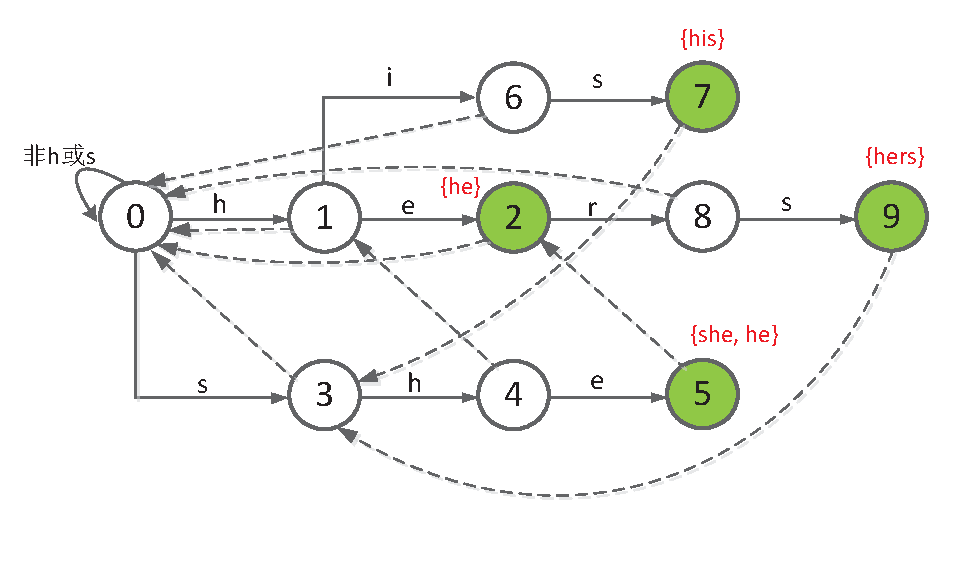
\includegraphics[height=7cm ,width=10cm]{figures/1_Introduction/AC.eps}
  \caption{为模式集$P=\{he, his, she, hers\}$所构建的AC自动机。}
  \label{fig:AC}
\end{figure}

2. \textbf{WM(Wu-Manber)算法}

 WM算法是BM算法在多模式环境下的推广,BM算法采用“坏字符”规则在文本中
进行跳跃,而由于模式串个数的增加,WM算法将采用“坏字符块”技术,增大了
文本串和模式串不匹配的可能性.从而增加了直接跳跃的机会。它还使用前缀表
进一步过滤不匹配的模式串,使算法获得了较高的运行效率。

在预处理时,算法会为模式集构建3个表结构:哈希表,跳转表和前缀表。 跳转
表用于在扫描文本串的时候,根据读入字符串决定可以跳过的字符数,如果相应的
跳跃值为0,则说明可能产生匹配,就要使用哈希表和前缀表进一步判断, 以决定有
哪些匹配候选模式, 并验证究竟是哪个或者哪些候选模式完全匹配。因此,在现
有的多模式匹配算法中,使用块字符、哈希技术和前缀特征表技术的WM算法通常
被认为具有较高的效率,在实际中被广泛使用。 对WM更加具体的阐述将在第6章
介绍WM的改进算法时一并介绍。

\section{后缀数组}


后缀数组 (Suffix Array, 简称SA),是由给定字符串的所有后缀按照字典序排列
所构成的数组, 由 Manber和Myers等人提出\cite{Manber1993}, 具有结构紧凑且
空间占用小的特点, 通常作为空间节省的后缀树 (Suffix Tree) 的替代品, 被广
泛地应用于全文索引 \cite{Strate2015,Fischer2017,Arroyuelo2014},数据压
缩\cite{Louza2015,Chien2015,Pradhan2016,Brisaboa2015} 等领域。

图\ref{fig:suffix}中分别显示了为字符串$bananas$所构建的后缀树以及后缀数
组。由于在给定字符串之后,每个后缀便可由其起始位置完全确定,所以后缀数
组中只需保留后缀的起始位置,相比于后缀树,能够极大的节省存储空间。


\begin{figure}[!h]
  \centering
  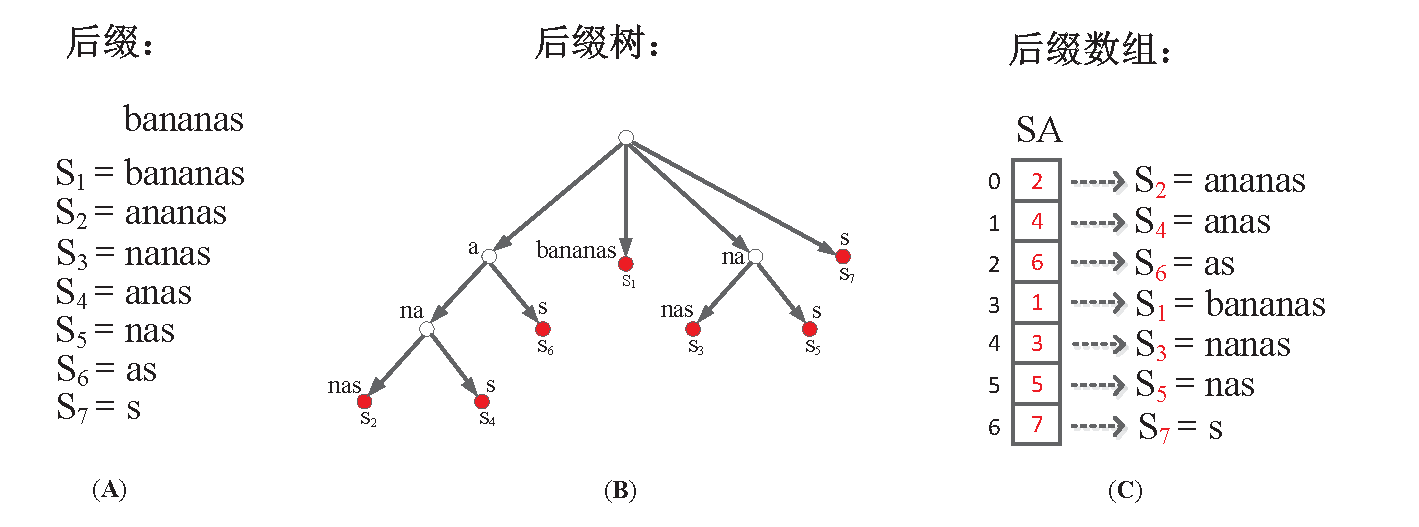
\includegraphics[height=7cm ,width=15cm]{figures/1_Introduction/Suffix.eps}
  \caption{(A) 字符串及其后缀。(B) 对应的后缀树。(C) 对应的后缀数组}
  \label{fig:Suffix}
\end{figure}

通过后缀树能完成的一些文本操作,同样可以通过后缀数组(及一些辅助结构)等
价地完成。例如,上一节中提到的单模式匹配问题,若模式串出现于文本串中,
它必定是某个(些)后缀的前缀,因此可以预先为文本串建立后缀树/数组,然后通
过在后缀树/数组上来查找模式串,可以在极短的时间内完成查找。举例来说,假
设文本串为$bananas$, 模式串为$an$, 对于后缀树,可以从其根节点开始,对模
式串进行逐字符遍历,之后发现有两个后缀即$S_3$与$S_5$都以$an$为前缀,因
此模式串$an$出现于文本串的第3和第5个位置,事实上利用后缀树进行单模式匹
配,可以在$O(m+c)$($m$为模式串长,
$c$为模式串在文本中出现的次数)时间内完成查讯操作。对于后缀数组,可以通
过后缀数组配合最长公共前缀数组,使用基于字典序的二分查找,能够
在$O(m+logn+c)$完成对模式串的搜索。因此,对那些不经常发生变化,且需要频
繁进行查询操作的文本,可以预先为其建立后缀数组(即文本索引),以加快查
询速度。

此外,有很多例子表明, 采用后缀数组比采用后缀树可获得更好的时间和空间空
性能。 例如, Pei\cite{Pei2013} 使用后缀树作为基本数据结构, 在字符串上寻
找最短唯一子串, 其时间复杂度为 $O(n^2)$。相比之下, Tsuruta
\cite{Tsuruta2014} 利用后缀数组和最长公共前缀数组作为基本数据结构, 将最
短唯一子串查询的时间复杂度降低到 $O(n)$, 而且空间方面也更节约。

很明显,构建后缀数组的过程本质上就是对后缀排序的过程。对后缀进行排序,
最直接的方法就是先对字符串按照字典序升序构造后缀树,然后对后缀树序深度
优先遍历后缀树,根据遍历到叶子节点的顺序来确定后缀的顺序。由于构造后缀
树具有线性时间复杂度的算法,因此理论上可以在线性时间内构造后缀数组。 然
而,这种间接地构造后缀数组的方法没有充分利用后缀数组的一些优于后缀树的
特性,不仅需要大量的存储空间,而且在实际中极其耗时。为此,应当研究直接
通过字符串文本构建后缀数组,而非间接地通过后缀树来排序。常见的直接构造
后缀数组的方法的有以下几种:

\subsection{DC3算法}
\label{sec:KA}

DC3 算法采用分治思想,与 Farach\cite{Farach1997}等人的线性时间后缀树构造
算法过程非常类似,其主要步骤为:

\begin{enumerate}
\item 以递归方式排序后缀$S_i$进行排序,这些后缀在字符串中的位
  置 $i$ 满足 $i mod 3 \neq 3$。 这使得字符串的规模缩减为原字符串
  的 2/3。
\item 对第一步所余下的后缀进行排序。
\item 合并步骤 1和步骤 2得到的结果。
\end{enumerate}

DC3 具有线性时间复杂度$O(n)$, $n$为字符串长度。其空间复杂度
为 $O(n/\sqrt{|\Sigma|})$(不包含输入字符串及建好的后缀数组所占空间),这
里$|\Sigma|$为字符集大小,且 $|\Sigma| \in [1, n]$。

\subsection{前缀倍增}

前缀倍增技术是实际应用当中广泛采用的后缀排序技术。其主要思想是由后缀的
首字符开始,逐步的来确定后缀之间的顺序,在第$k$轮中可以根据前$2^k$个字
符来对后缀进行排序,因此对长为$n$的字符串,最多需要$logn$轮,即可完成排
序十分的高效。举例来说,假设需要对字符串$bananas$的后缀进行排序。首先,
根据首字符对后缀进行排序,可将所有后缀分为4组,如
图\ref{fig:Prefix_Doubling}(A)所示。其中,组间有序而组内无序,即第1组中
的$S_6$, $S_4$,
$S_2$由于其首字符相同,此时还无法确定顺序,类似地,第3组中
的$S_5$和$S_3$也暂时无法确定顺序。由于$S_6$, $S_4$,
$S_2$首字符相同,因此它们之间的顺序取决于后面的字符串即$s$, $nas$,
$nanas$之间的顺序,这恰好是$S_7$, $S_5$,
$S_3$,由于$S_7$是字典序最大的后缀,所以$S_6$将大于$S_4$与$S_2$,又由
于$S_5$,
$S_3$次序待定,所以$S_4$与$S_2$次序待定。类似地,对于第3组中
的$S_5$和$S_3$,其顺序将由$S_6$与$S_4$决定,由于$S_6$大于$S_4$,$S_5$将
大于$S_3$,如图\ref{fig:Prefix_Doubling}(B)所示。最后,
第1组中$S_4$和$S_2$的顺序将取决于$S_6$和$S_4$, 由于$S_6$大于$S_4$,因
此,$S_4 $大于$S_2$,如图\ref{fig:Prefix_Doubling}(C)所示,排序完成。

\begin{figure}[!h]
  \centering
  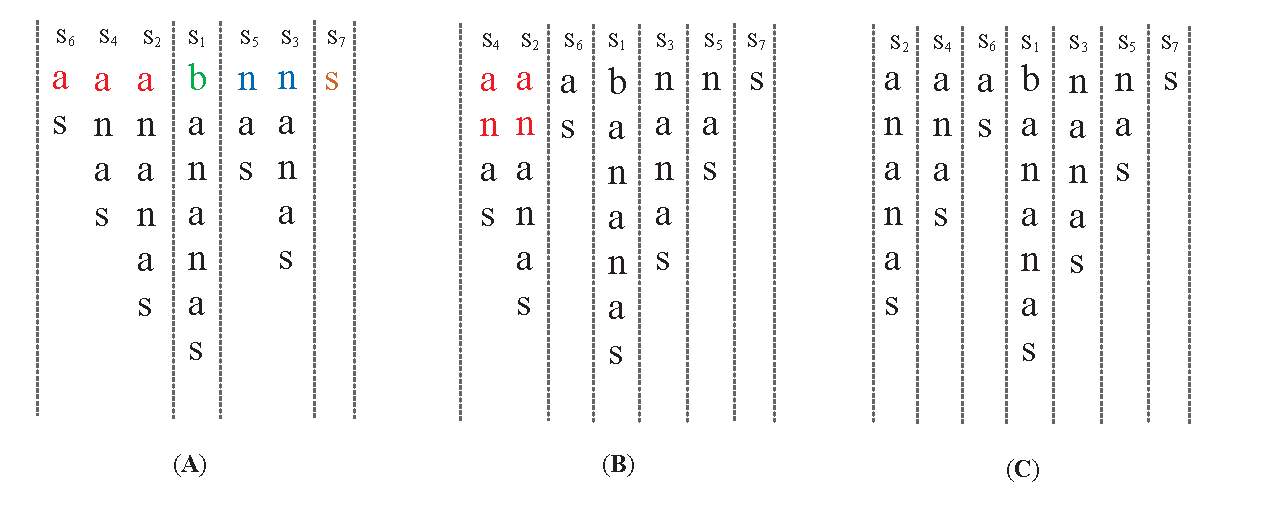
\includegraphics[height=6cm ,width=15cm]{figures/1_Introduction/Prefix_Doubling.eps}
  \caption{利用前缀倍增技术对$bananas$的后缀进行排序。(A) 第一轮。(B) 第二轮。(C) 第三轮。}
  \label{fig:Prefix_Doubling}
\end{figure}




\section{最长公共子序列}

度量生物序列间的相似性是生物信息学中的一类基本问题,它们在癌症检
测\cite{Aravanis2017,Chattopadhyay2016,Munday2017},探寻物种的共同起
源 \cite{Zvelebil2007,Perry2015,Donnell2015} 等许多方面具有广泛的应用。
度量序列间相似性最重要手段之一是寻找序列间的最长公共子序列 (Longest
Common Subsequence,简称为LCS), 这已被证实是一类NP难问
题\cite{Maier1978}。根据目标序列的个数,该问题可以被分为两类:(1)寻找两
个序列的最长公共子序列被称为最长公共子序列(LCS)问题;(2) 寻找超过两个序
列的最长公共子序列被称为多最长公共子序列(MLCS)问题。


\begin{figure}[!h]
  \centering
  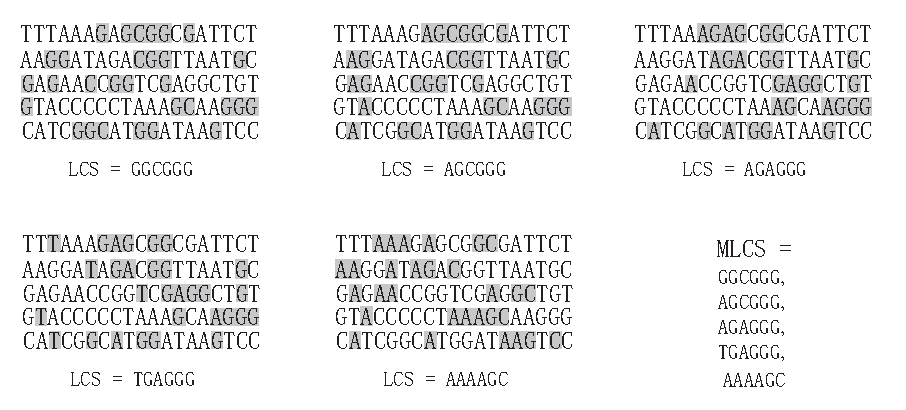
\includegraphics[height=6cm ,width=15cm]{figures/1_Introduction/MLCS.eps}
  \caption{5个DNA序列的最长公共子序列。}
  \label{fig:MLCS}
\end{figure}


给定序列集,通常会存在多个最长公共子序列。如图 \cite{fig:MLCS}所示,给
定5个长为19的DNA序列,存在4个长为6的最长公共子序列。



\section{本文主要工作及内容安排}
\label{sec:org}

本文针对序列挖掘领域中的三个重要问题:(1) 多模式匹配问题;(2)后缀排序问
题;(3) 最长公共子序列问题,进行了研究,分别提出(或改进)了几种高效的
算法。

本文的主要内容安排如下:

第二章首先介绍了多模式匹配问题的概念及相关工作。然后,针对现有的基于内
存的多模式匹配算法为模式集所构造的数据结构鲁棒性较差,性能易受到模式集
自身特性(尤其是最短模式串长)的影响,同时可伸缩性较差,在处理大规模模式
集时,性能往往无法满足实际需求,提出了一种高效的多模式匹配引擎。 接着,
介绍了该引擎包括过滤与核实两个模块:过滤模块基于位图结构,所有操作均基
于底层位运算,因此能够快速地过滤掉文本串中不可能出现匹配的位置;对每一
个潜在的匹配位置,调用核实模块来确认是否有模式串出现。 核实模块基于一种
被称为“自适应匹配树”的树形结构,树中的每个节点都保存了模式集的一部分
片段,节点内部的存储结构将根据自身所保存的模式集片段的特征(即片段长度和
片段数量)进行自适应地调整,以达到时间效率和空间效率的最佳平衡。 由于每
个节点的自适应性,使得对于任何特性的模式集,所构造的自适应匹配树都能够
保持最高效的形态。然后,给出了三种进一步优化的技术:分解自适应匹配树,
节点合并以及节点分裂。将大的自适应匹配树分解成多个小的树结构,可以提高
匹配时的命中率,同时节约内存;节点合并可以将多个单支节点合并为一个节点,
提高算法的运行效率,同时节省内存开销。节点分裂能够减少不必要的比较操作,
进一步提高匹配速度。最后,从鲁棒性和可伸缩性两方面将所提方法和现有方法
进行了对比实验,证明了其具有较好的鲁棒性和伸缩性, 尤其对于大规模模式
集。

第三章首先介绍了后缀排序问题及其相关研究工作。然后介绍了广泛使用的前缀
倍增排序算法---qsufsort算法。针对传统的qsufsort算法存在的缺陷:在每一轮
排序中,所有后缀都将依据定长前缀(即在第$k$轮中,根据每个后缀长为$2^k$的
后缀)被排序,这意味着前$2^k$个字符都相同的后缀,无法在第$k$轮中被确定顺
序,这样,对于那些具有很长公共前缀的后缀,需要许多轮才能被确定顺序。提
出了一种改进型的后缀排序算法---dsufsort,dsufsort算法将记录并维护后缀数
组中每个未排序桶的深度,在每一轮排序中,将根据待排序桶的深度对其中的后
缀进行排序,这使得在第$k$轮中,后缀可以基于长度超过$2^k$的前缀被排序,从
而那些前$2^k$个字符相同的后缀便可在第$k$轮中被确定顺序, 因
此,dsufsort算法仅需要较少的轮数就可以完成排序。 此外,由于桶的深度具有
累加性,因此,对于具有很长公共前缀的后缀,dsufsort算法可以更快速地完成
排序。接着给出了dsufsort算法一些高效的实现技巧,包括:提前对输入字符串
进行输入变化,在第一轮中采用桶排序对后缀进行排序,以及选择合适的排序函
数。最后,通过实验与现有的算法进行了比较,试验结果证实,对于绝大多数情
况,dsufsort算法的性能要优于现有算法。

第四章首先介绍了最长公共子序列问题及其研究现状。然后介绍了现有的两种两
种解决方案:基于动态规划的方法和基于支配点图模型的方法。 针对现有的基于
支配点图的方法,在构建图时会产生大量的节点,导致内存过度消耗,同时,在
大规模图中搜索最长路径,以构建最长公共子序列会花费较长的运行时间的问题,
提出了一种新的层次化图模型---Leveled-DAG,及其相应的构建算法。 不同于现
有的算法在构造有向无环图时,需要保存所有产生的节点,并在图构造好之后通
过搜索其中的最长路径来构建相应的最长公共子序列, Leveled-DAG模型可以在
建图的过程中实时地构建目标序列的最长公共子序列,并及时删除那些对构建最
长公共子序列没有任何影响的无用节点。在任一时刻,Leveled-DAG只需保存最新
产生的一层节点以及前面产生的入度不为0的节点,并且,随着构建过程的进行,
图中的节点数将会逐渐减少,最终将仅剩余一个节点,所有目标序列的最长公共
子序列都保存在该节点中。 最后,将所提出的图模型与现有的方法进行了实验对
比, 得益于实时地构造最长公共子序列及删除无用节点,所提模型相比现有算法
在时间和空间效率上都有较大提升。

第五章对WM多模式匹配算法进行改进。首先介绍了WM算法的基本思想与算法流程,
然后对其进行了两方面的改进:(1) 通过寻找每个模式串中出现频率最少的字符
块来确定该模式的特征串,以这样的特征串来构造Hash表避免了出现过长哈希链
的情况,并可将频繁遍历的哈希链中的模式串转移到其它哈希链中,减少了程序
运行中精确匹配的次数,该方法对于包含较短模式的模式集以及模式集和文本相
互有关联的情况,效果尤为明显;(2) 通过为较长的哈希链建立一个索引表,并
通过在该索引表上的二分查找,算法可以在极短的时间内找到需要精确匹配的模
式串,避免了对整条哈希链的遍历,随着模式集规模的增加该方法效果愈加明
显。最后,通过实验证实了改进算法相比原始WM在性能上有较大提升。

第六章对全文进行了总结与展望。
